\section{结构相关化合物与可迁移变量}

\begin{figure}[t]
  \centering
  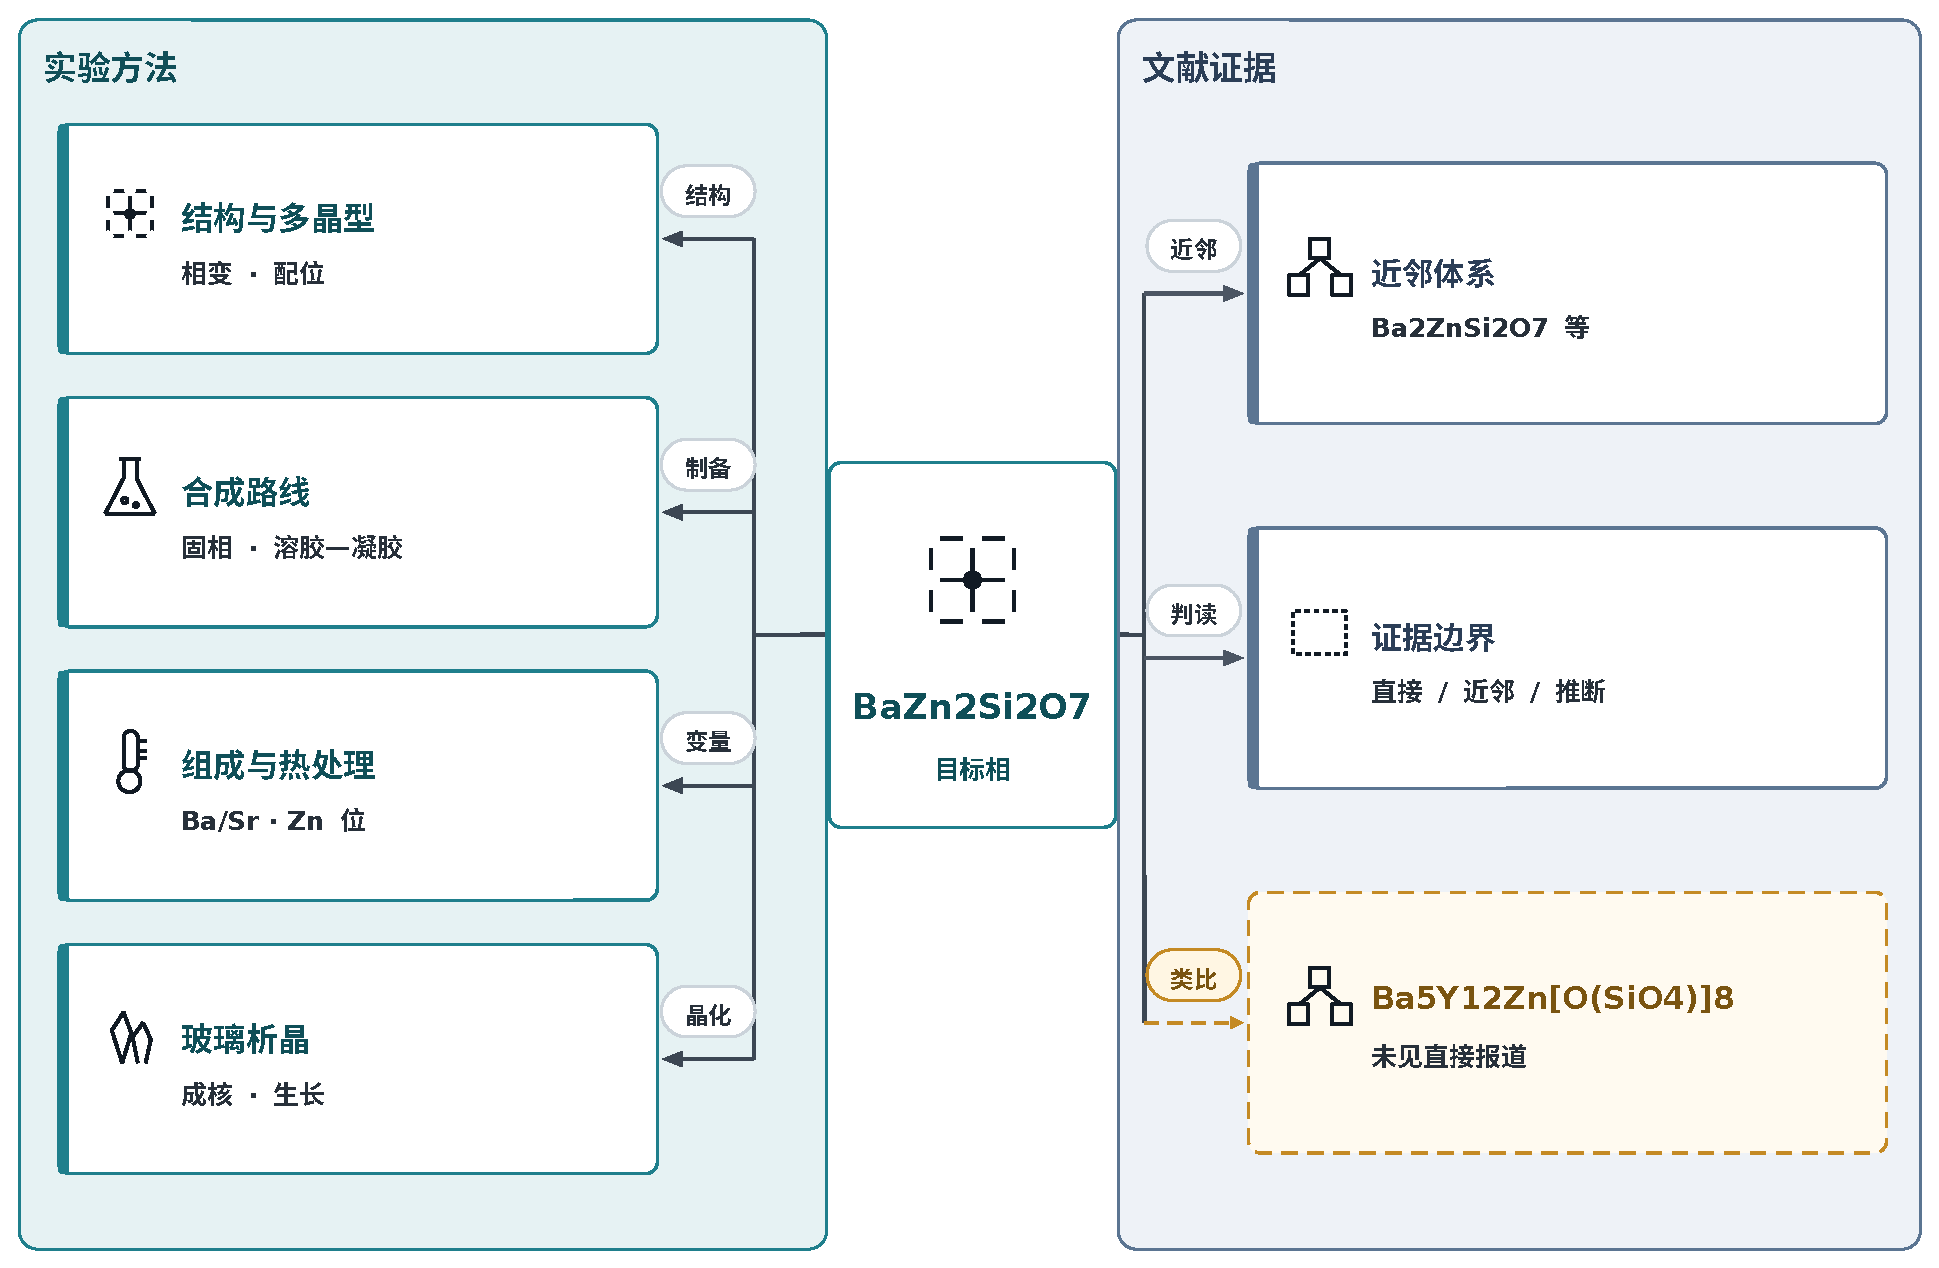
\includegraphics[width=\linewidth]{../figures/pdf/taxonomy_phase_control.pdf}
  \caption{\textbf{BaZn$_2$Si$_2$O$_7$ 合成与相控制的分类框架。}实线分支表示目标相的直接实验依据或结构相关化合物的实验依据，虚线节点表示尚无直接结构报道的比较对象。}
  \label{fig:taxonomy}
\end{figure}

\subsection{Ba\slash Sr 取代}

Ba$_{1-x}$Sr$_x$Zn$_2$Si$_2$O$_7$ 是研究最充分的同构取代体系。Sr$^{2+}$ 取代 Ba$^{2+}$ 可降低高温相的形成温度；取代量超过约 10\% 时，高温结构可保留至室温，并表现出近零或负热膨胀 \cite{thieme2015ba1,thieme2016very,thieme2017variable,zou2021near}。单晶 XRD 将该稳定相确定为正交 Cmcm，ZnO$_4$ 链的扭曲和摆动被认为是负热膨胀的重要结构来源 \cite{thieme2015ba1}。上述结果表明，A 位离子尺寸和多面体空隙是相控制的有效变量，但不能据此推断 Y$^{3+}$ 可大量进入同一位点。

\subsection{Zn 位与 Si 位取代}

Mg、Co、Mn、Ni、Cu 等二价离子可在不同范围内取代 Zn。取代量超过临界值时，低温结构可能重新出现，表明局域配位偏好与长程相稳定性之间存在竞争 \cite{thieme2016new,kerstan2013bazn2si2o7}。Ge 取代 Si 则通过四面体尺寸和键柔性改变相变温度；不含 Sr 的组成中 Ge 固溶度有限，而含 Sr 组成可将高温结构保持至更高的 Ge 含量 \cite{thieme2016negative}。

\subsection{微晶玻璃工艺}

玻璃路线的研究表明，动力学因素与化学组成同等重要。Pt 成核剂促进异质成核，Nb$_2$O$_5$\slash Ta$_2$O$_5$ 改变表面析晶与体析晶的比例，贵金属还可能形成合金或核壳结构 \cite{vladislavova2017heterogeneous,heitmann2019surface,thieme2022noble,thieme2018growth}。晶粒尺寸低于约 80~\textmu m 时，微裂纹减少，宏观热膨胀更接近晶体本征值 \cite{thieme2016thermal}。因此，BaZn$_2$Si$_2$O$_7$ 的相控制研究应同时报告相组成、晶粒尺寸和裂纹状态。
